\begin{frame}{Self-Attention Mechanism}
  \begin{itemize}
    \item[$\blacktriangleright$] Computes contextual representation of a word using all other words
    \item[$\blacktriangleright$] \textbf{Inputs:} Query (Q), Key (K), Value (V)
    \item[$\blacktriangleright$] \textbf{Output:} Weighted sum of values
  \end{itemize}

  \vspace{0.5em}
  \textbf{Attention formula:}
  \begin{align*}
    \text{Attention}(Q, K, V) = \mathrm{softmax}\left(\frac{QK^T}{\sqrt{d_k}}\right)V
  \end{align*}

  \vspace{0.5em}
  \begin{itemize}
    \item[$\blacktriangleright$] Enables each word to attend to all others
  \end{itemize}
\end{frame}

\begin{frame}{Self-Attention Intuition: The ``Bank'' Analogy}
  \begin{itemize}
    \item[$\blacktriangleright$] \textbf{Query:} What we're looking for (e.g., the meaning of ``bank'' in context)
    \item[$\blacktriangleright$] \textbf{Keys:} Tags or features associated with each word/sentence (e.g., ``river'', ``money'')
    \item[$\blacktriangleright$] \textbf{Values:} Information linked to each key (e.g., context-specific meaning)
    \item[$\blacktriangleright$] Uses dot-product similarity between Query and Keys to assign attention weights
    \item[$\blacktriangleright$] Weighted sum of Values produces the contextual representation
  \end{itemize}
\end{frame}

\begin{frame}{Self Attention}
  \centering
  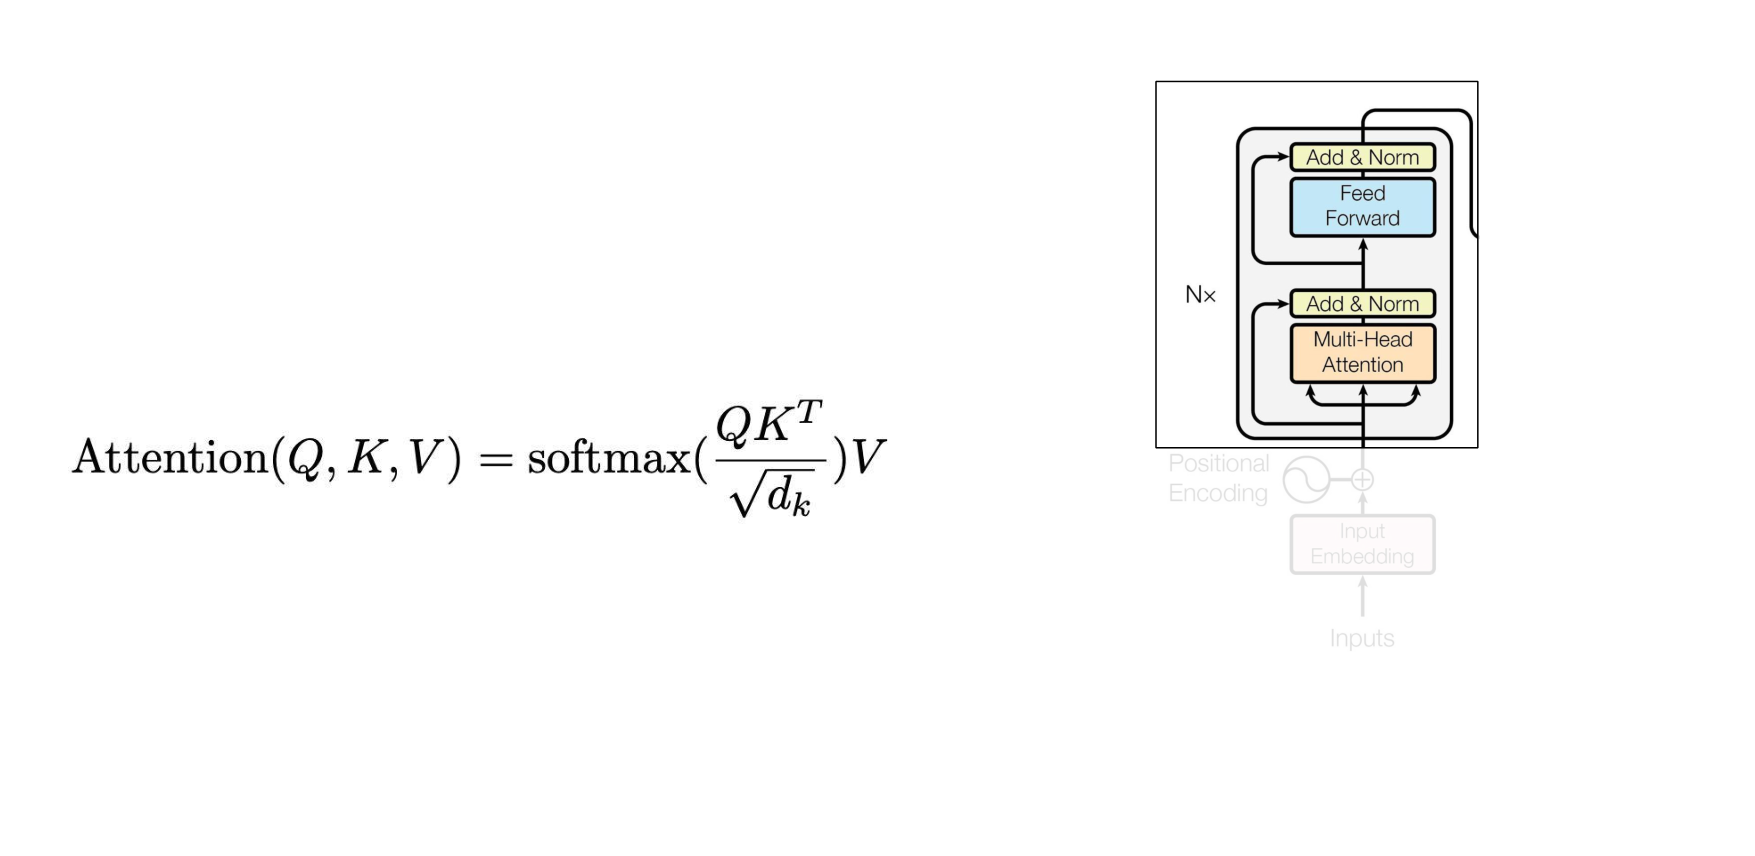
\includegraphics[width=0.9\paperwidth,height=0.75\paperheight,keepaspectratio]{images/introduction-to-transformers/transformer_attention_formula_with_encoder_diagram.png}

  {\scriptsize Source: CMU 11-785, Lecture 19 ``Transformers,'' Spring 2024, slide 33.}
\end{frame}

\begin{frame}{Self Attention}
  \centering
  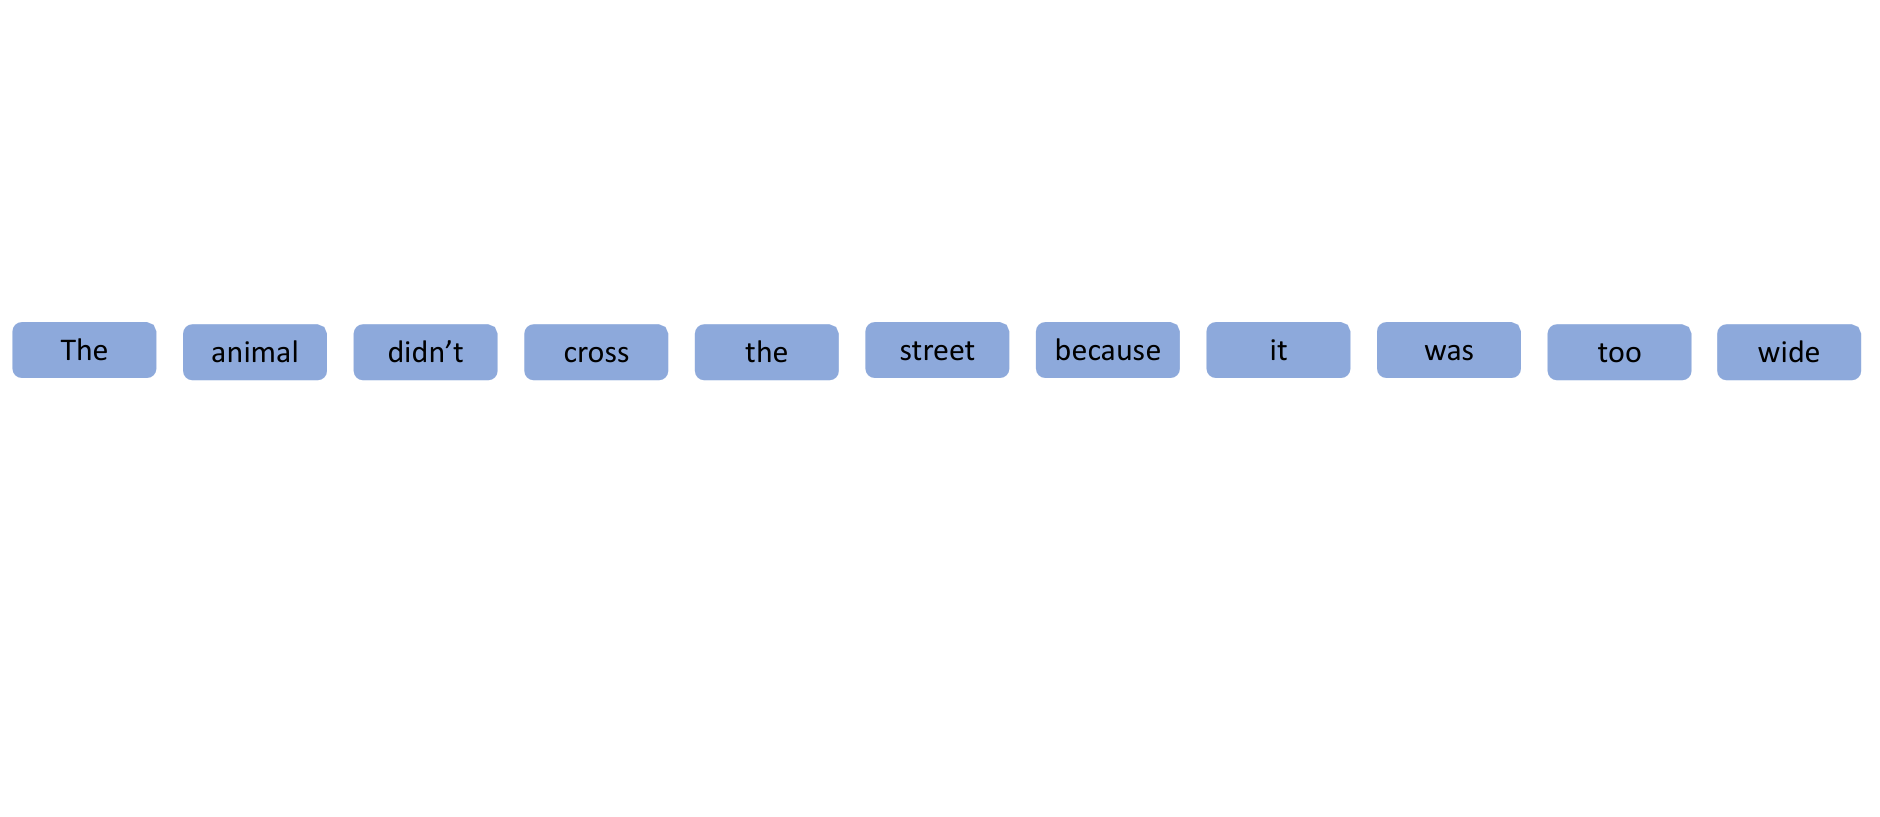
\includegraphics[width=\linewidth,height=0.75\paperheight,keepaspectratio]{images/introduction-to-transformers/transformer_example_sentence_tokens.png}

  {\scriptsize Source: CMU 11-785, Lecture 19 ``Transformers,'' Spring 2024, slide 61.}
\end{frame}

\begin{frame}{Self Attention}
  \centering
  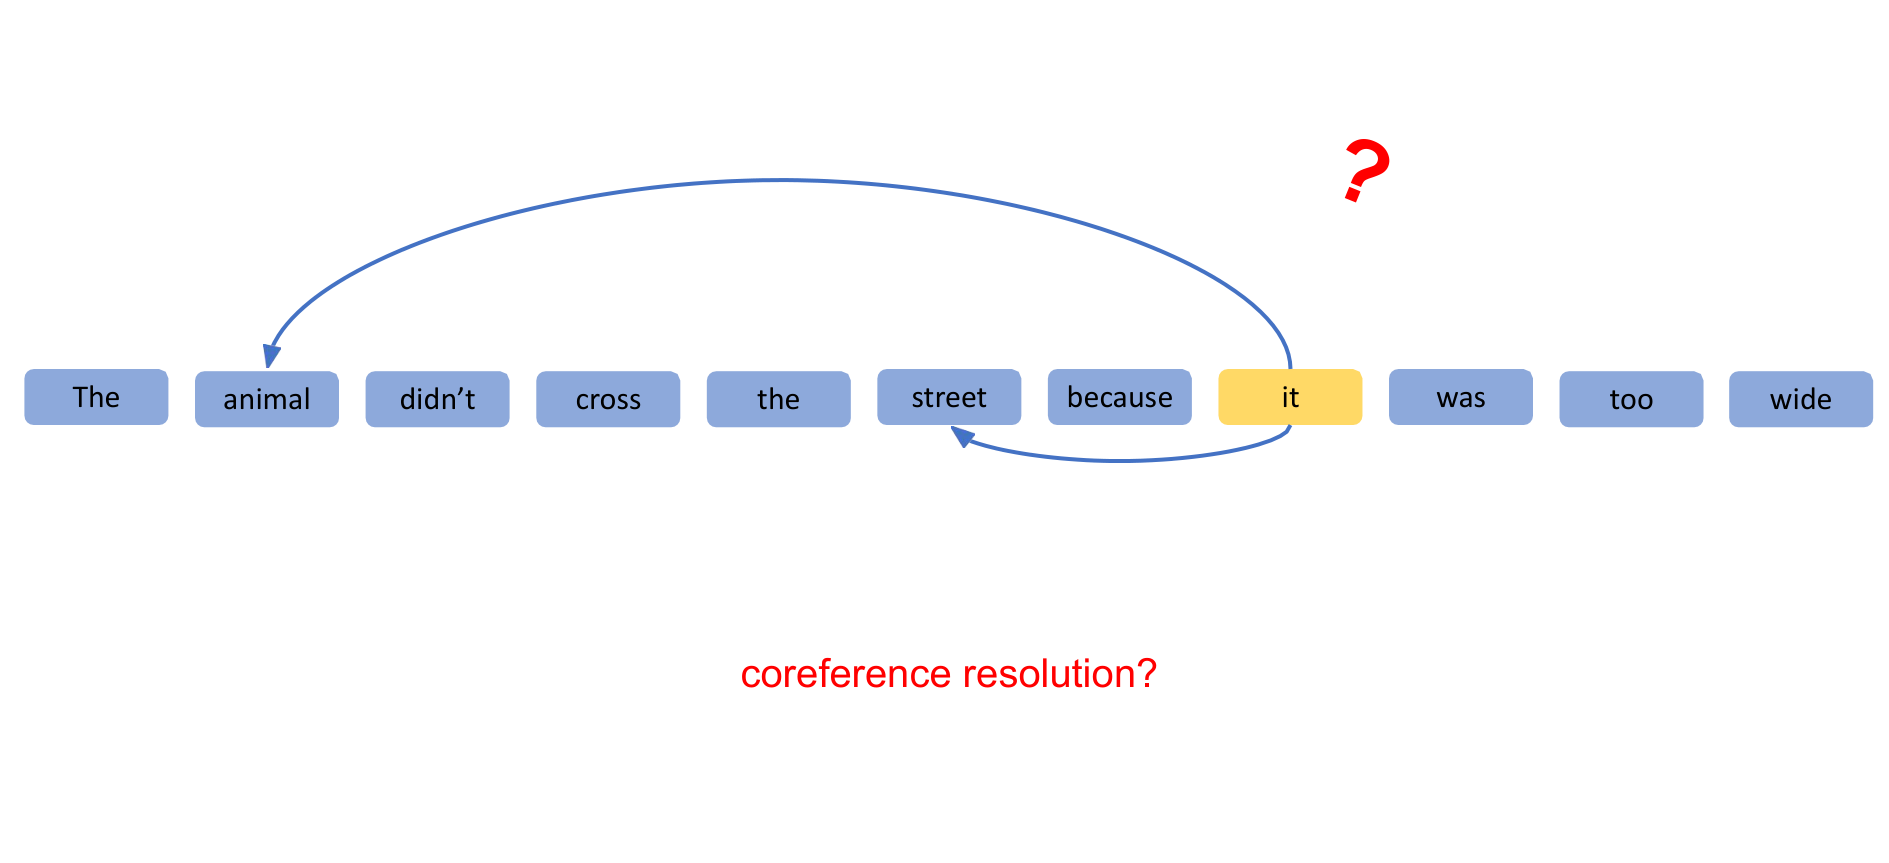
\includegraphics[width=\linewidth,height=0.75\paperheight,keepaspectratio]{images/introduction-to-transformers/transformer_coreference_resolution_it_question.png}

  {\scriptsize Source: CMU 11-785, Lecture 19 ``Transformers,'' Spring 2024, slide 62.}
\end{frame}

\begin{frame}{Self Attention}
  \centering
  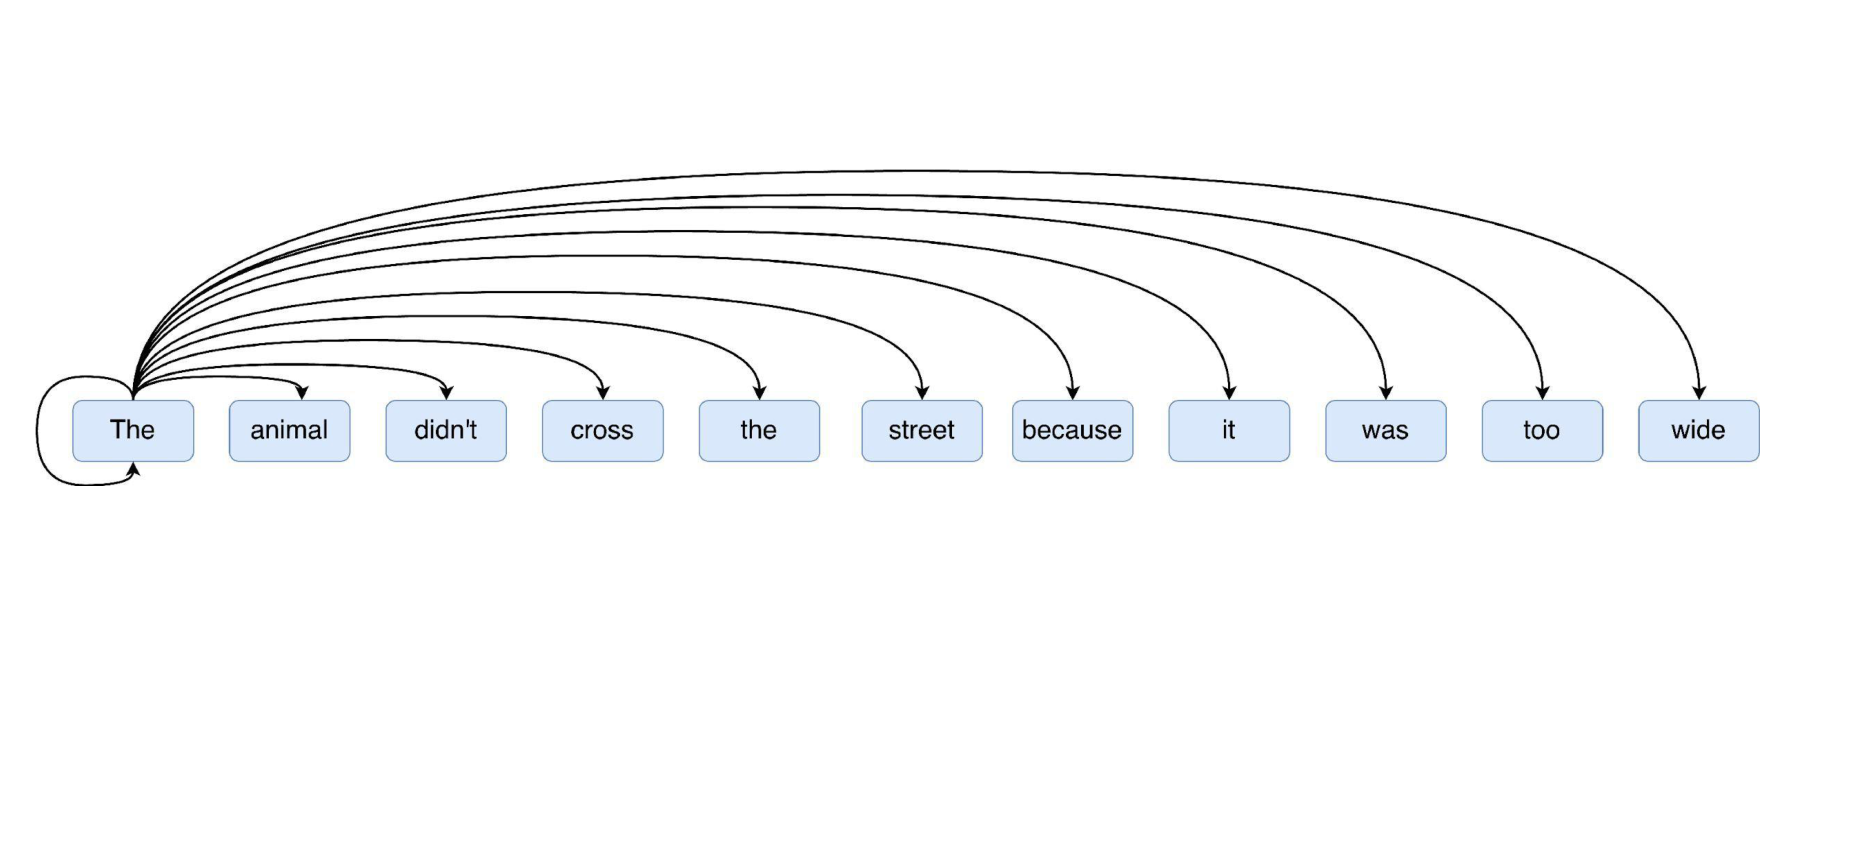
\includegraphics[width=\linewidth,height=0.75\paperheight,keepaspectratio]{images/introduction-to-transformers/transformer_self_attention_the_to_all_words.png}

  {\scriptsize Source: CMU 11-785, Lecture 19 ``Transformers,'' Spring 2024, slide 63.}
\end{frame}

\begin{frame}{Self Attention}
  \centering
  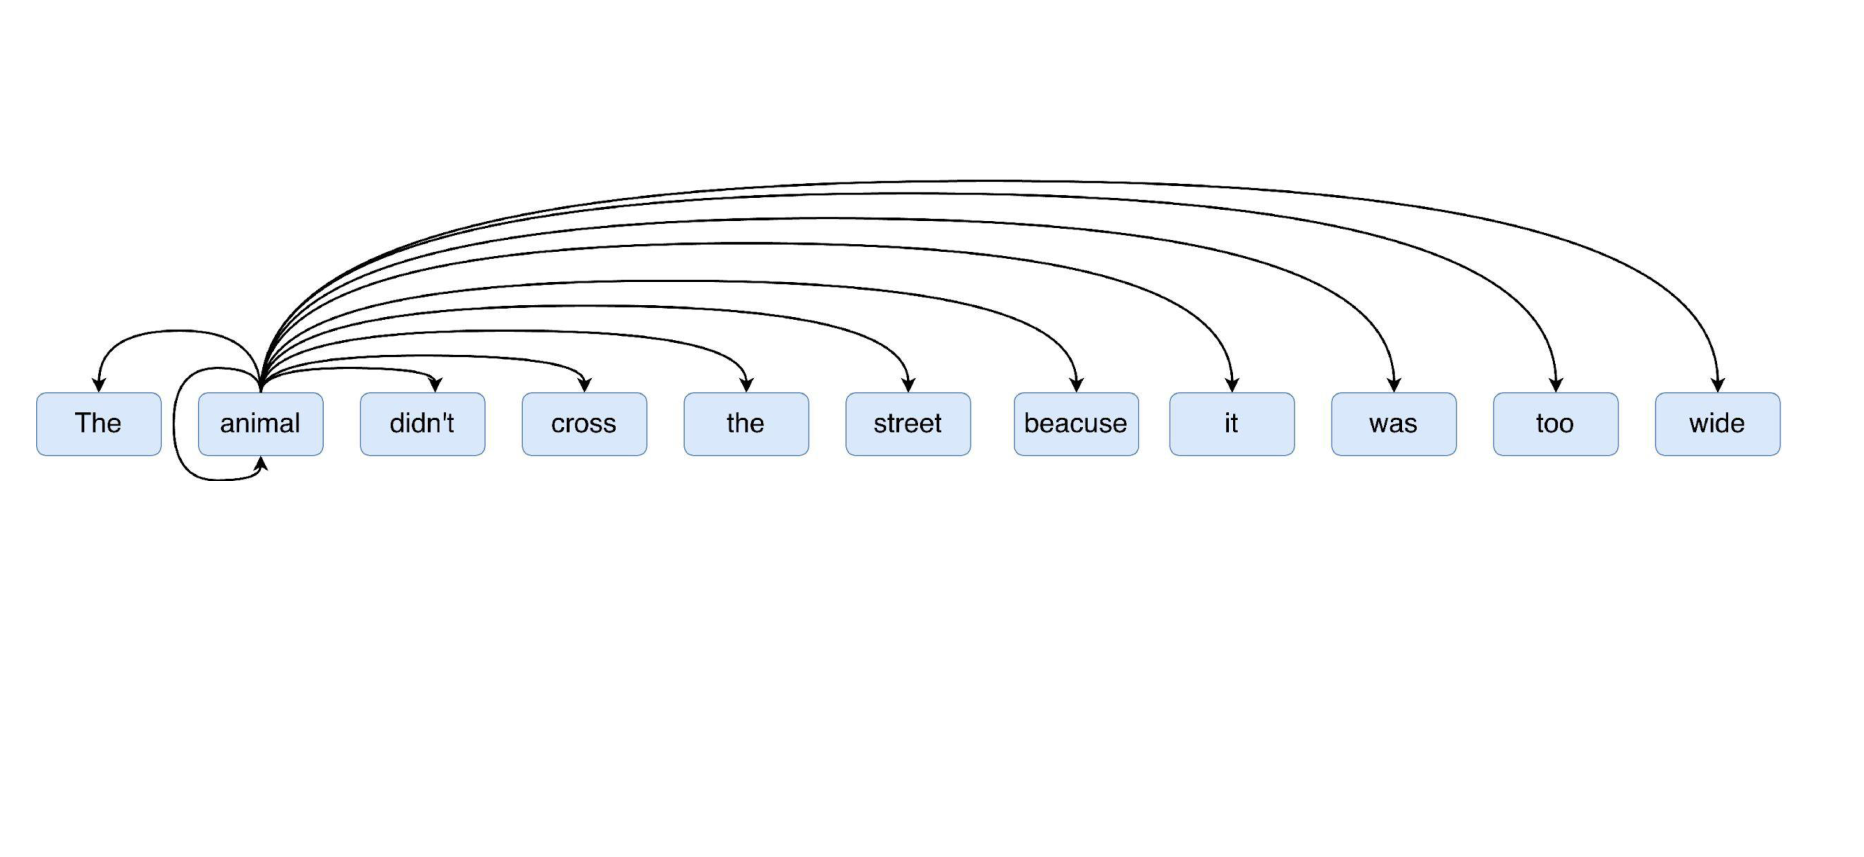
\includegraphics[width=\linewidth,height=0.75\paperheight,keepaspectratio]{images/introduction-to-transformers/transformer_self_attention_animal_to_all_words.png}

  {\scriptsize Source: CMU 11-785, Lecture 19 ``Transformers,'' Spring 2024, slide 64.}
\end{frame}

\begin{frame}{Self Attention}
  \centering
  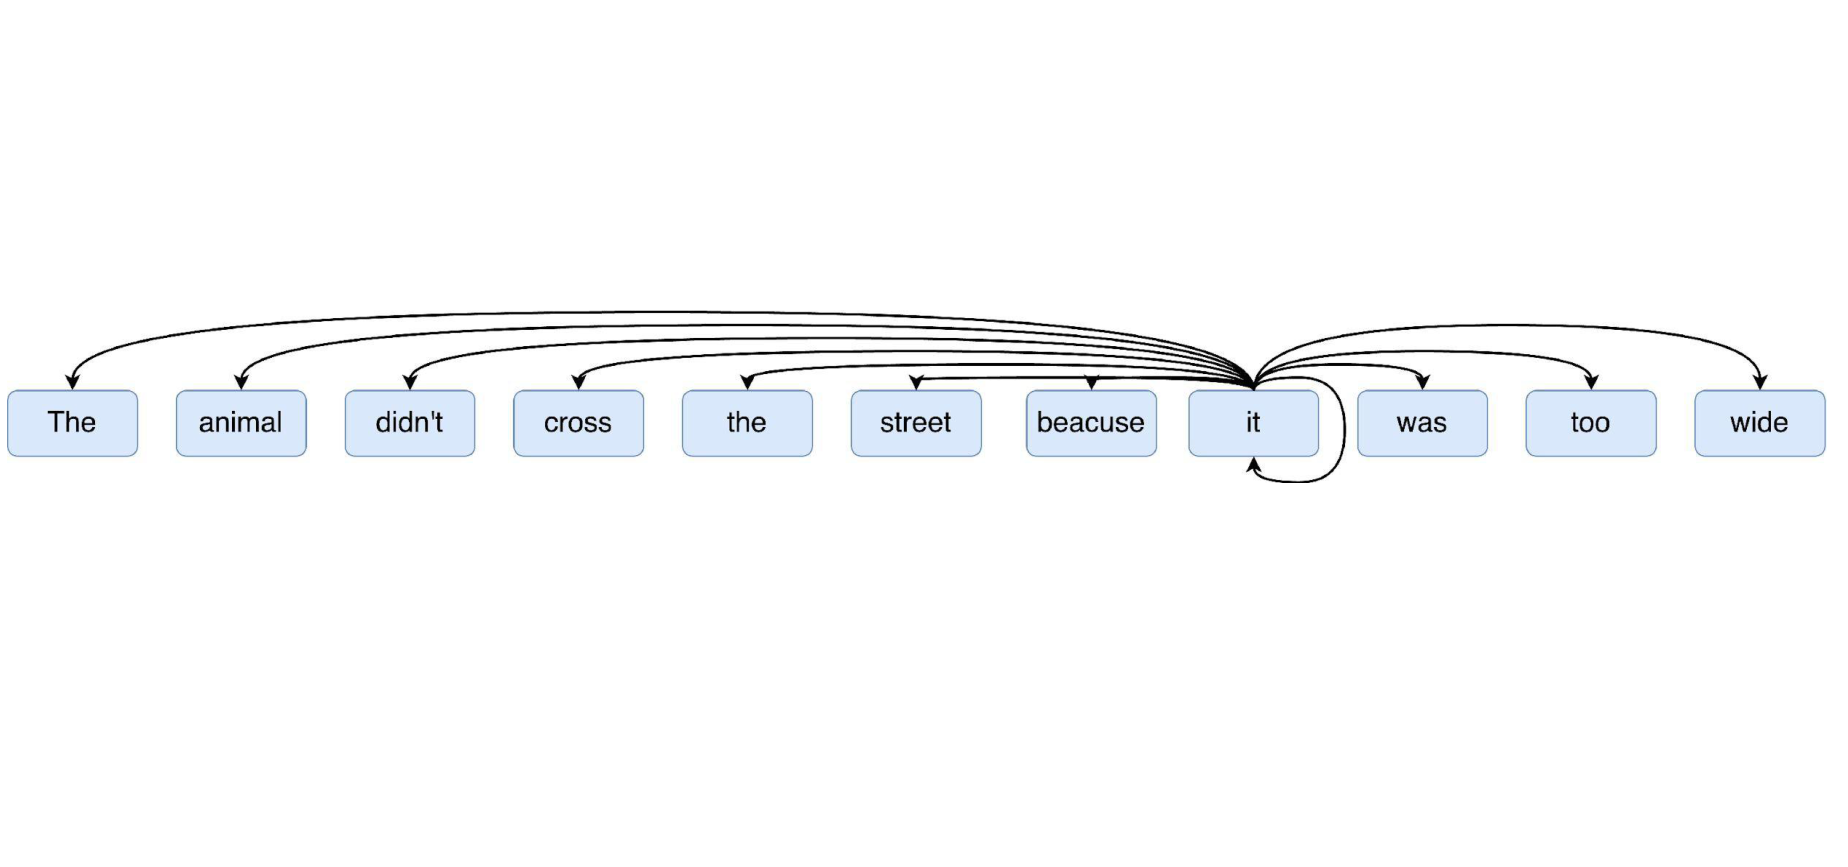
\includegraphics[width=\linewidth,height=0.75\paperheight,keepaspectratio]{images/introduction-to-transformers/transformer_self_attention_it_to_all_words.png}

  {\scriptsize Source: CMU 11-785, Lecture 19 ``Transformers,'' Spring 2024, slide 65.}
\end{frame}

\begin{frame}{Self Attention}
  \centering
  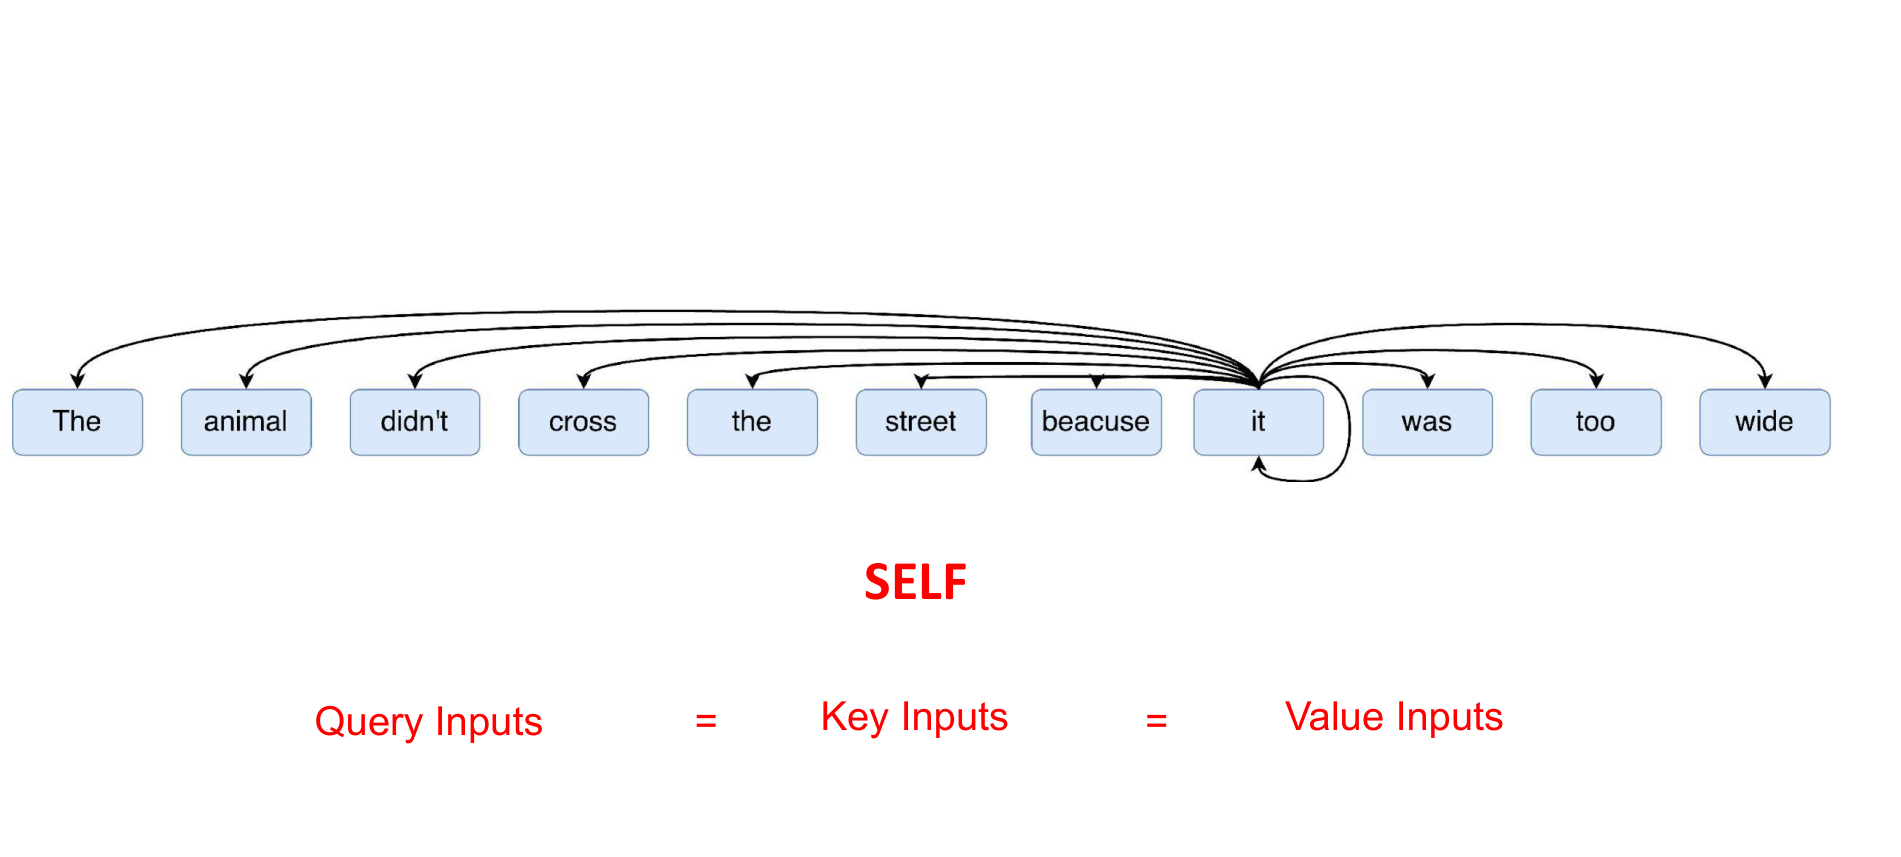
\includegraphics[width=\linewidth,height=0.75\paperheight,keepaspectratio]{images/introduction-to-transformers/transformer_self_attention_qkv_same_inputs.png}

  {\scriptsize Source: CMU 11-785, Lecture 19 ``Transformers,'' Spring 2024, slide 66.}
\end{frame}

\begin{frame}{Self Attention}
  \centering
      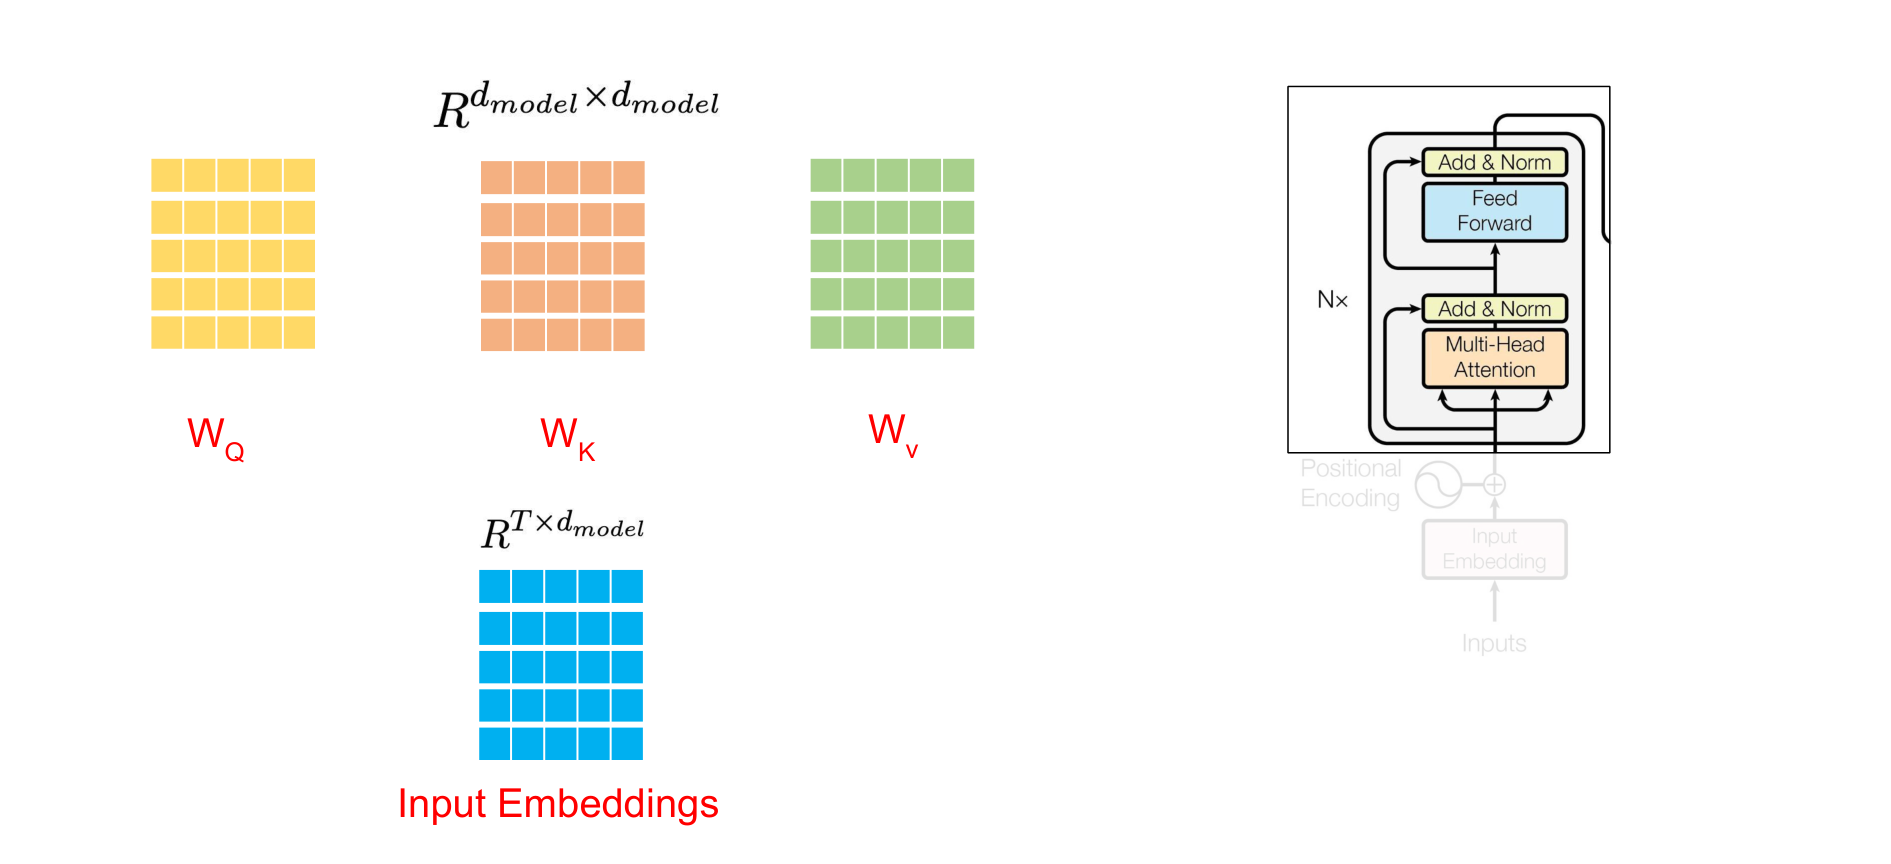
\includegraphics[width=\linewidth,height=0.75\paperheight,keepaspectratio]{images/introduction-to-transformers/transformer_weight_matrices_wq_wk_wv_and_embeddings.png}

      {\scriptsize Source: CMU 11-785, Lecture 19 ``Transformers,'' Spring 2024, slide 67.}
\end{frame}

\begin{frame}{Self Attention}
  \centering
  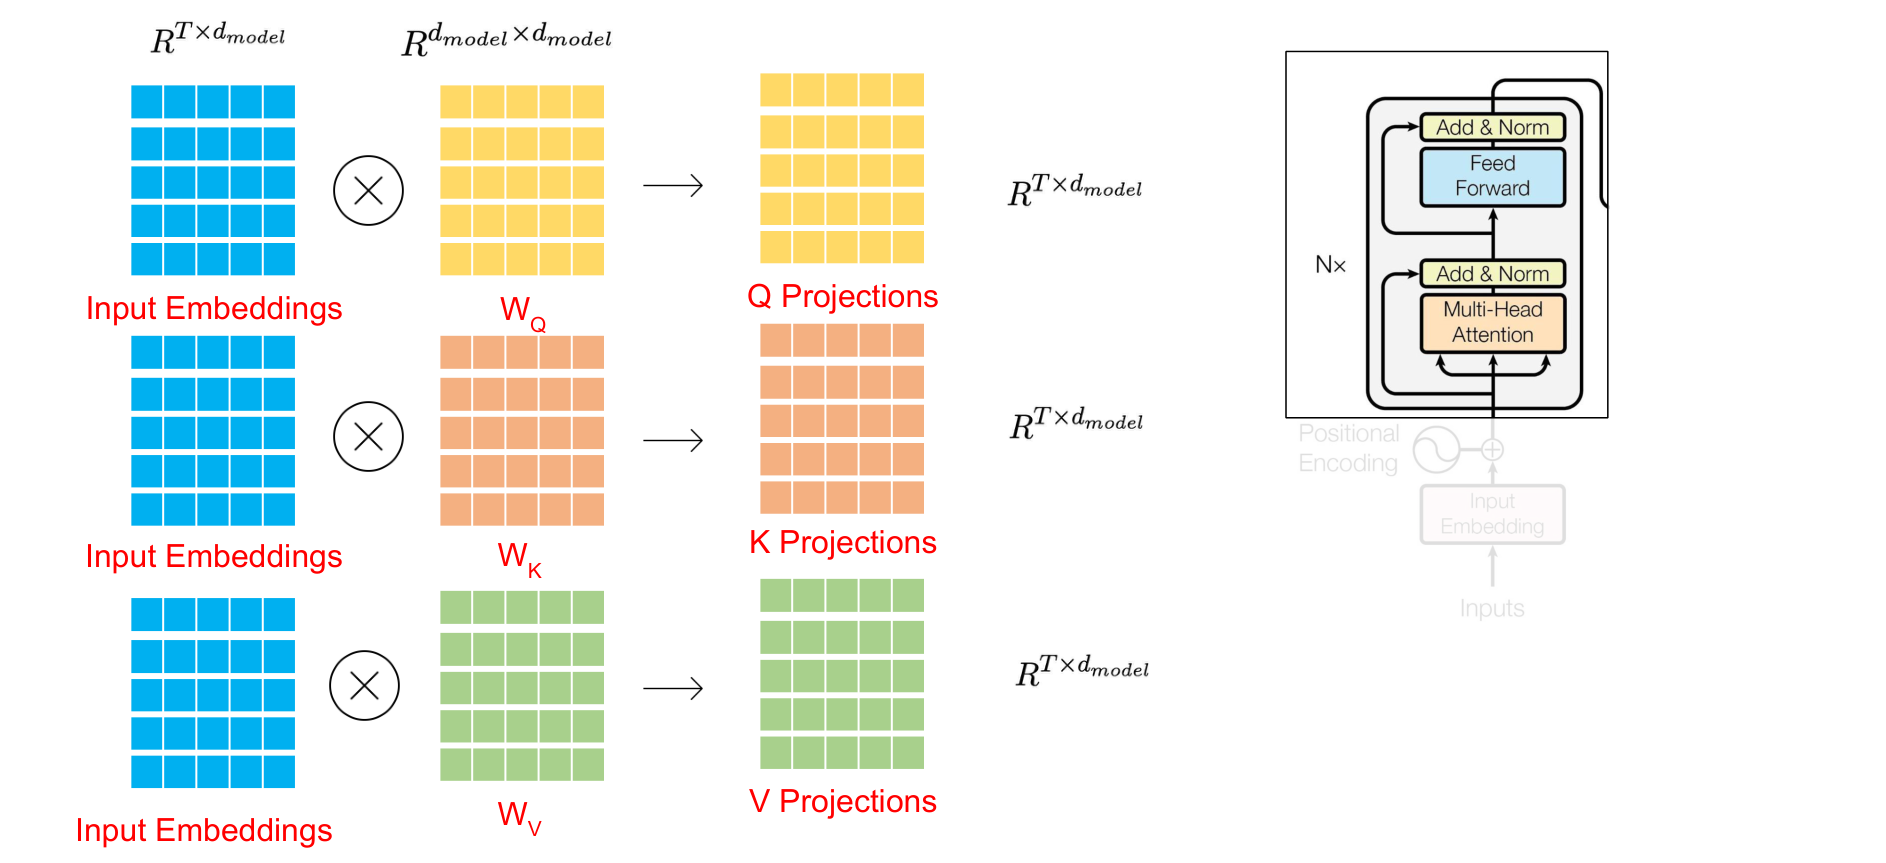
\includegraphics[width=\linewidth,height=0.75\paperheight,keepaspectratio]{images/introduction-to-transformers/transformer_qkv_projections_from_embeddings.png}

  {\scriptsize Source: CMU 11-785, Lecture 19 ``Transformers,'' Spring 2024, slide 68.}
\end{frame}

\begin{frame}{Self Attention}
  \centering
  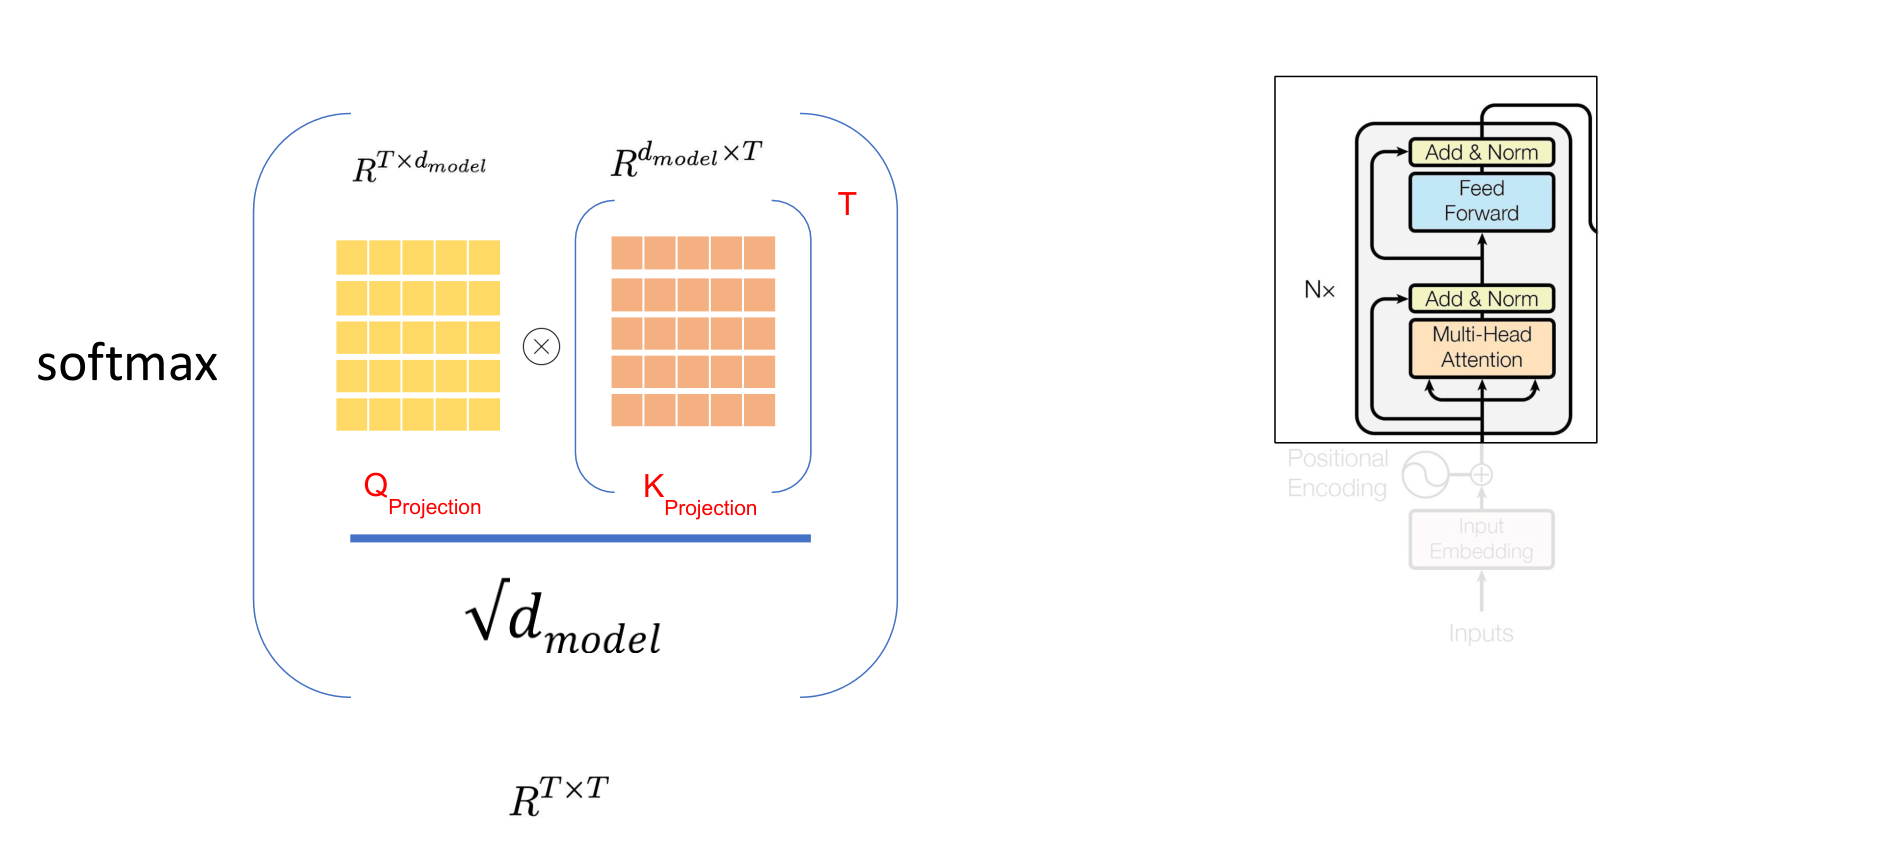
\includegraphics[width=\linewidth,height=0.75\paperheight,keepaspectratio]{images/introduction-to-transformers/transformer_softmax_qk_transpose_scaled.png}

  {\scriptsize Source: CMU 11-785, Lecture 19 ``Transformers,'' Spring 2024, slide 69.}
\end{frame}

\begin{frame}{Self Attention}
  \centering
  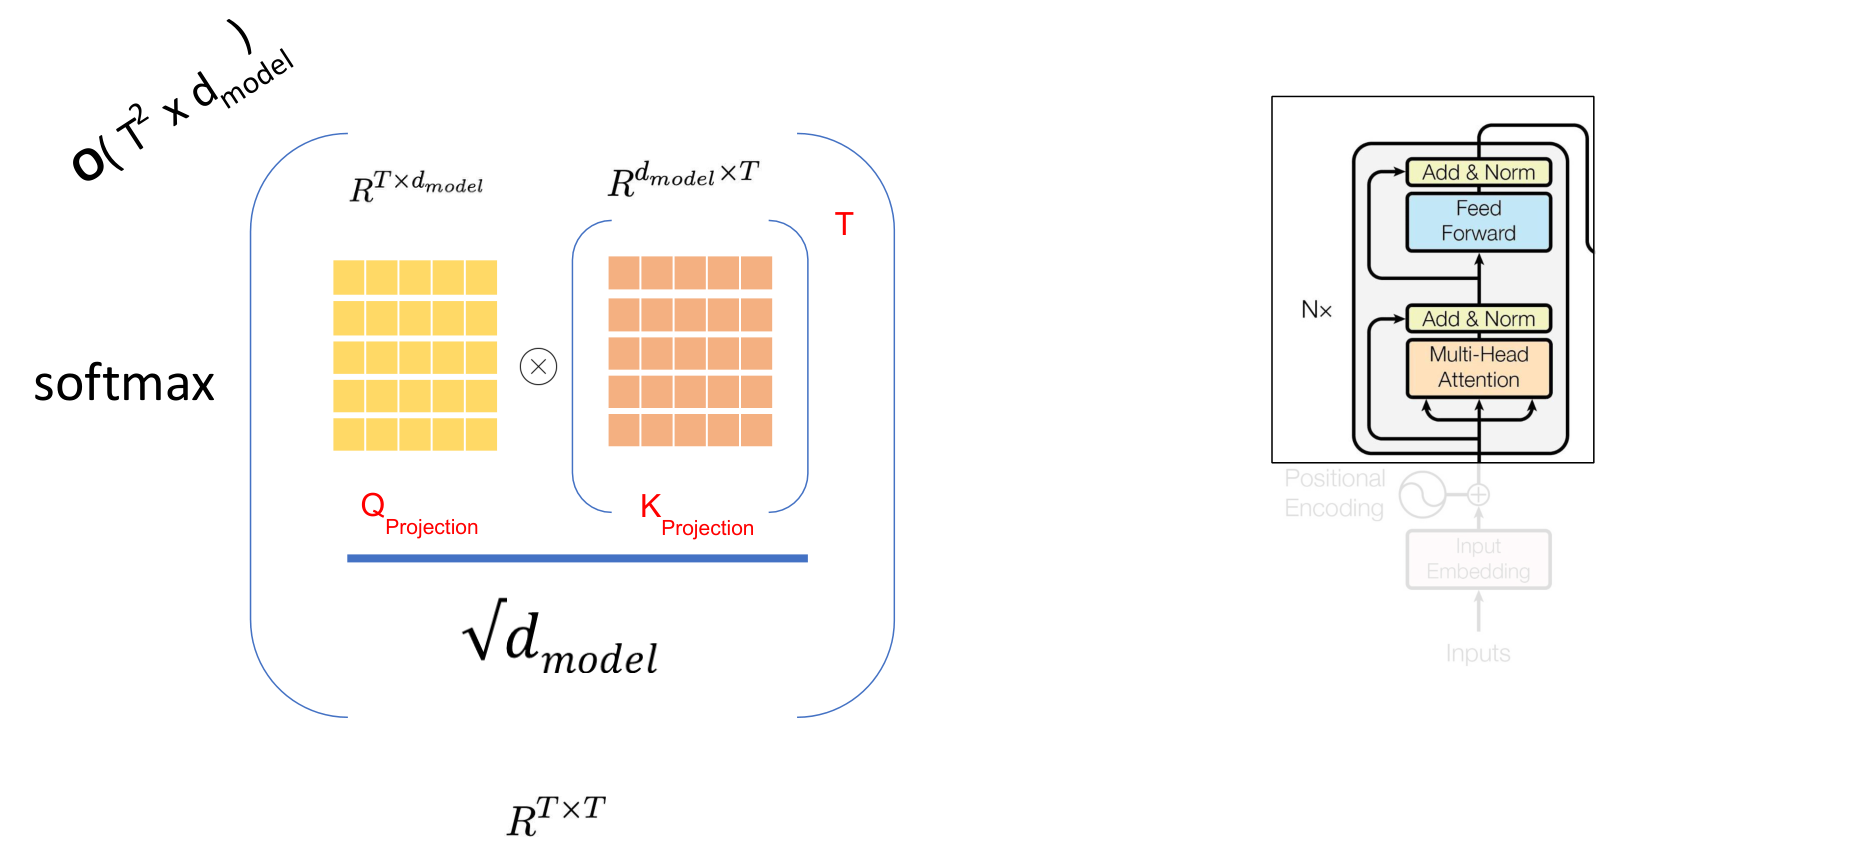
\includegraphics[width=\linewidth,height=0.75\paperheight,keepaspectratio]{images/introduction-to-transformers/transformer_softmax_qk_complexity_annotation.png}

  {\scriptsize Source: CMU 11-785, Lecture 19 ``Transformers,'' Spring 2024, slide 70.}
\end{frame}

\begin{frame}{Self Attention}
  \centering
  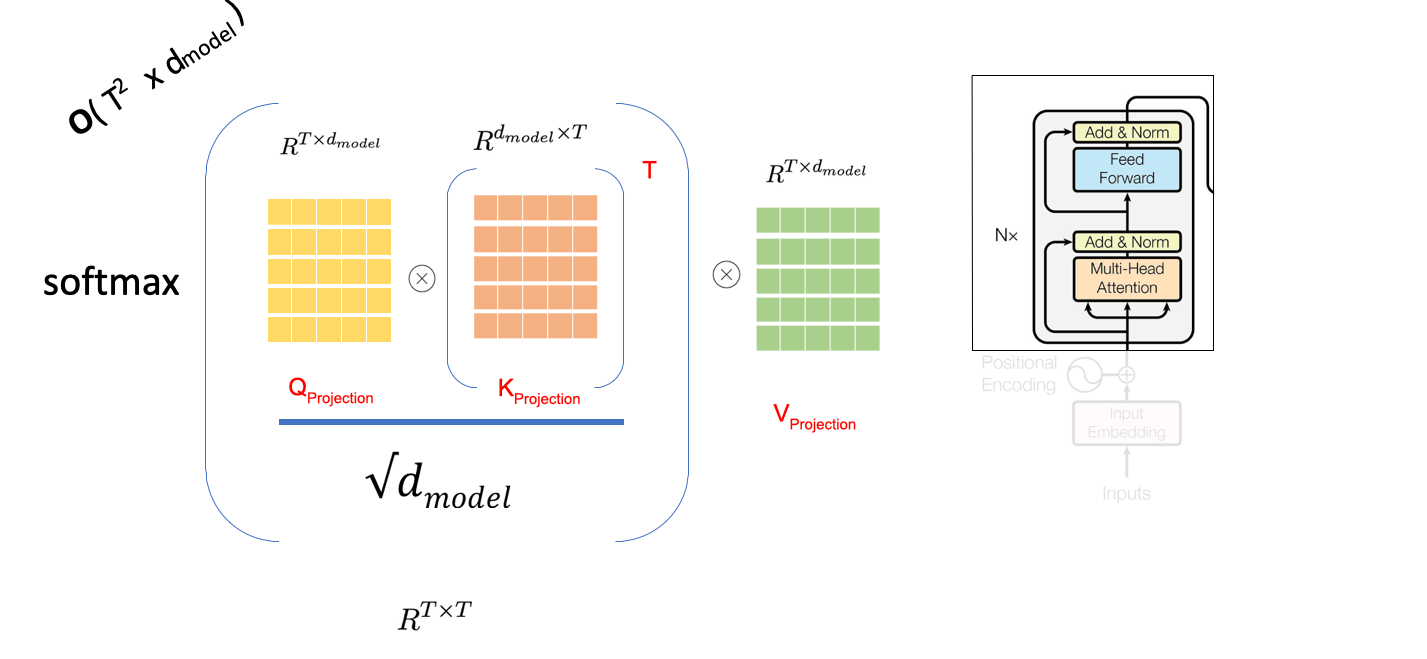
\includegraphics[width=\linewidth,height=0.75\paperheight,keepaspectratio]{images/introduction-to-transformers/transformer_softmax_qk_times_v_projection.png}

  {\scriptsize Source: CMU 11-785, Lecture 19 ``Transformers,'' Spring 2024, slide 71.}
\end{frame}

\begin{frame}{Self Attention}
  \centering
  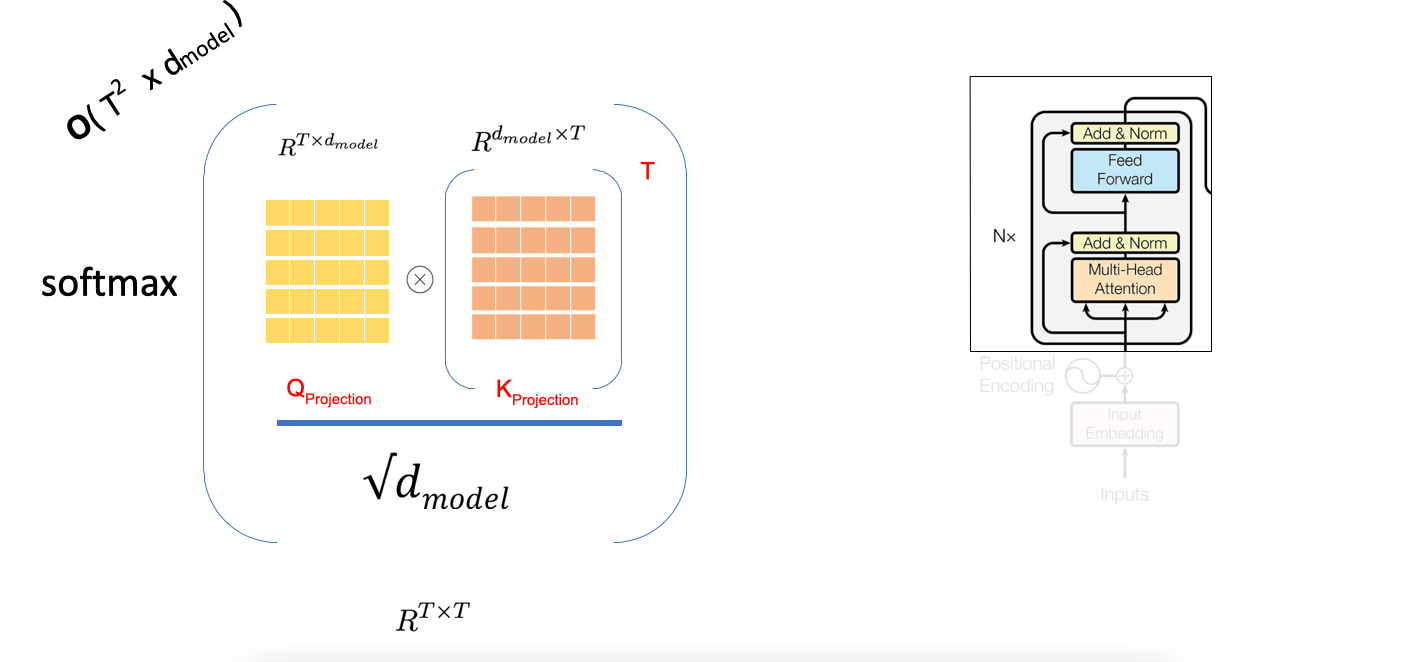
\includegraphics[width=\linewidth,height=0.75\paperheight,keepaspectratio]{images/introduction-to-transformers/transformer_softmax_qk_transpose_encoder_highlighted.png}

  {\scriptsize Source: CMU 11-785, Lecture 19 ``Transformers,'' Spring 2024, slide 72.}
\end{frame}

\begin{frame}{Self Attention}
  \centering
  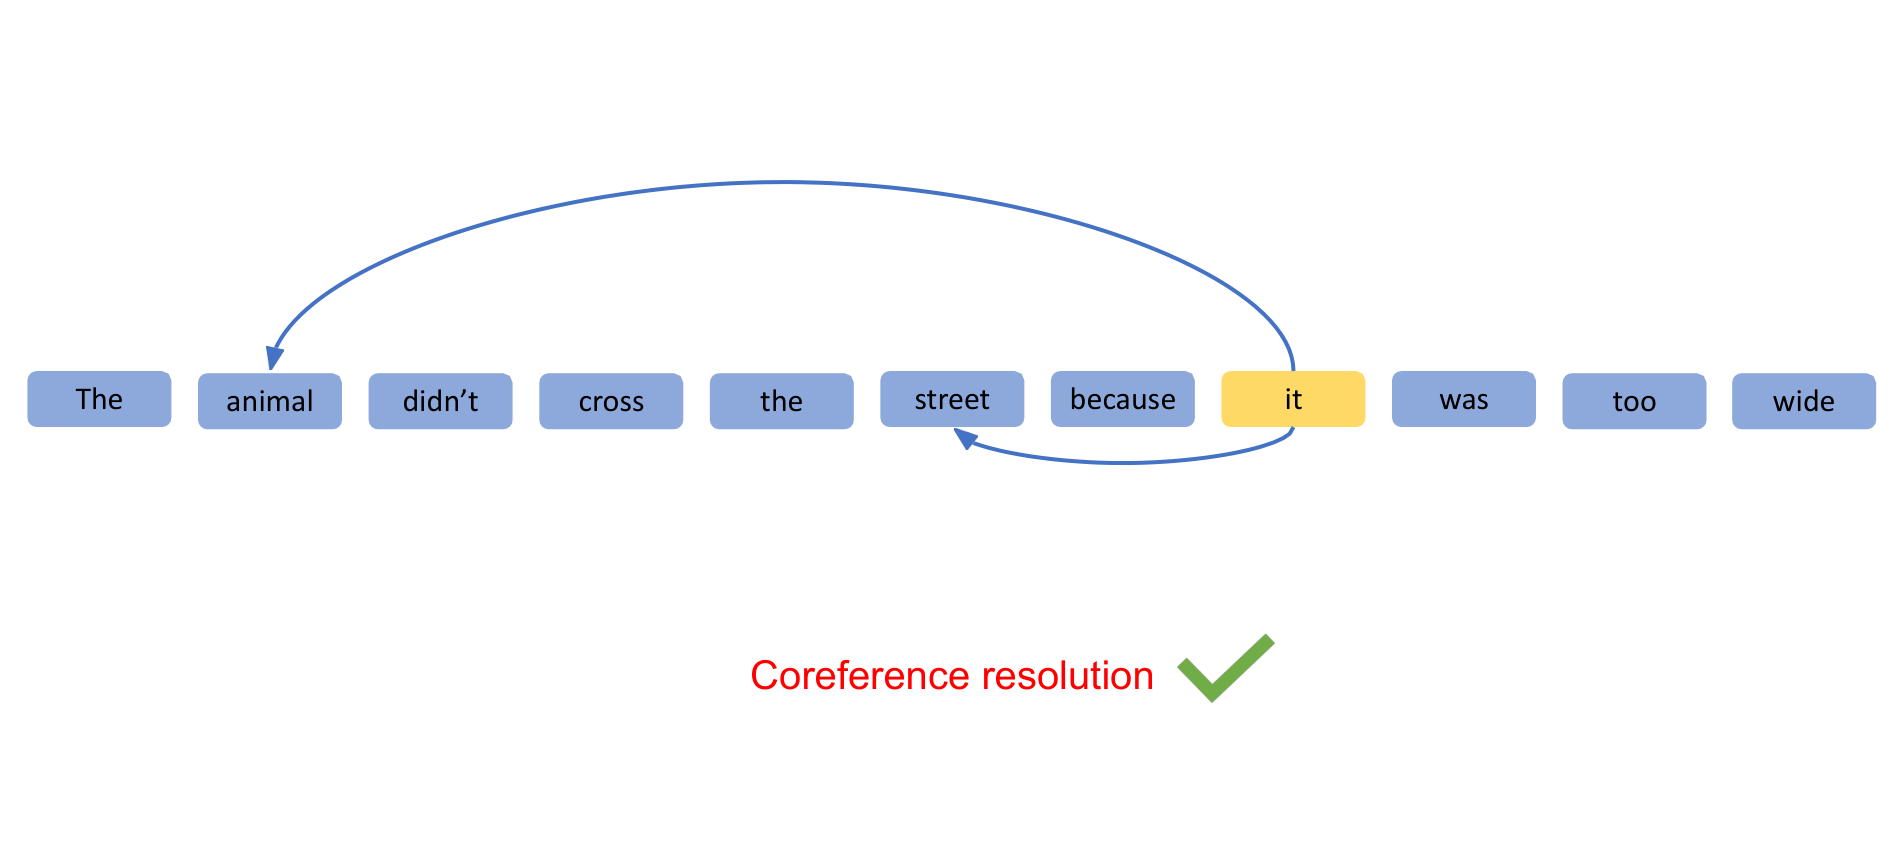
\includegraphics[width=\linewidth,height=0.75\paperheight,keepaspectratio]{images/introduction-to-transformers/transformer_coreference_resolution_solved_checkmark.png}

  {\scriptsize Source: CMU 11-785, Lecture 19 ``Transformers,'' Spring 2024, slide 73.}
\end{frame}

\begin{frame}{Self Attention}
  \centering
  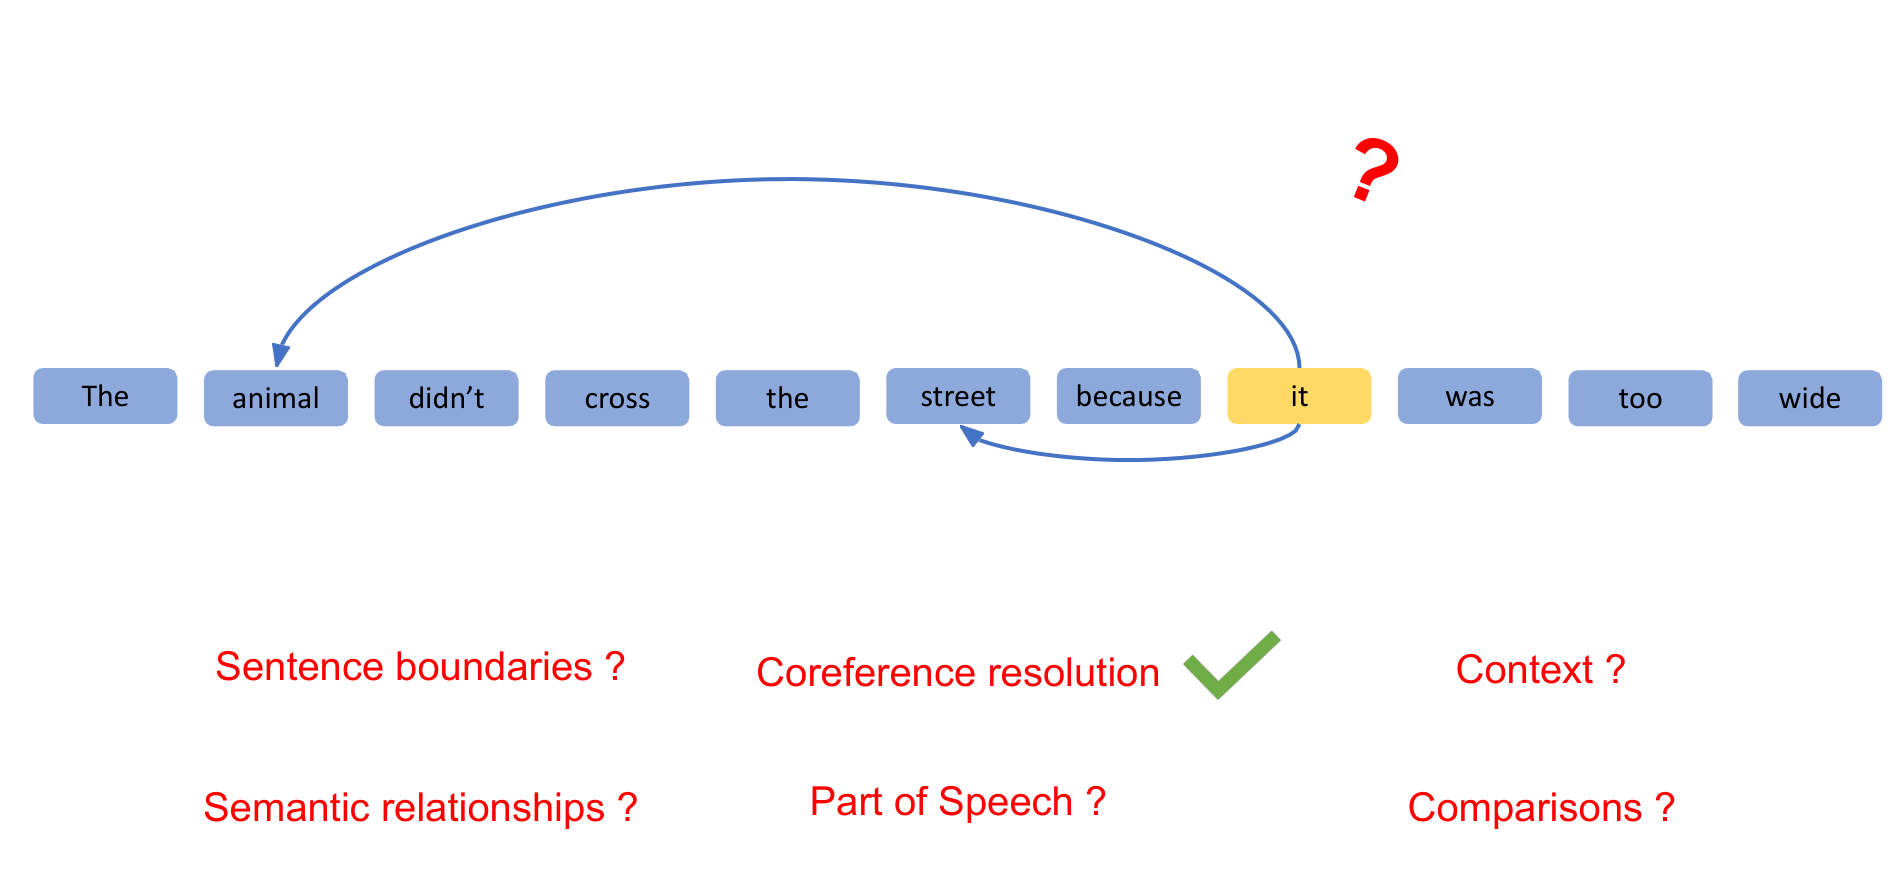
\includegraphics[width=\linewidth,height=0.75\paperheight,keepaspectratio]{images/introduction-to-transformers/transformer_nlp_tasks_questions_coreference_solved.png}

  {\scriptsize Source: CMU 11-785, Lecture 19 ``Transformers,'' Spring 2024, slide 74.}
\end{frame}

\begin{frame}{Self Attention}
  \centering
  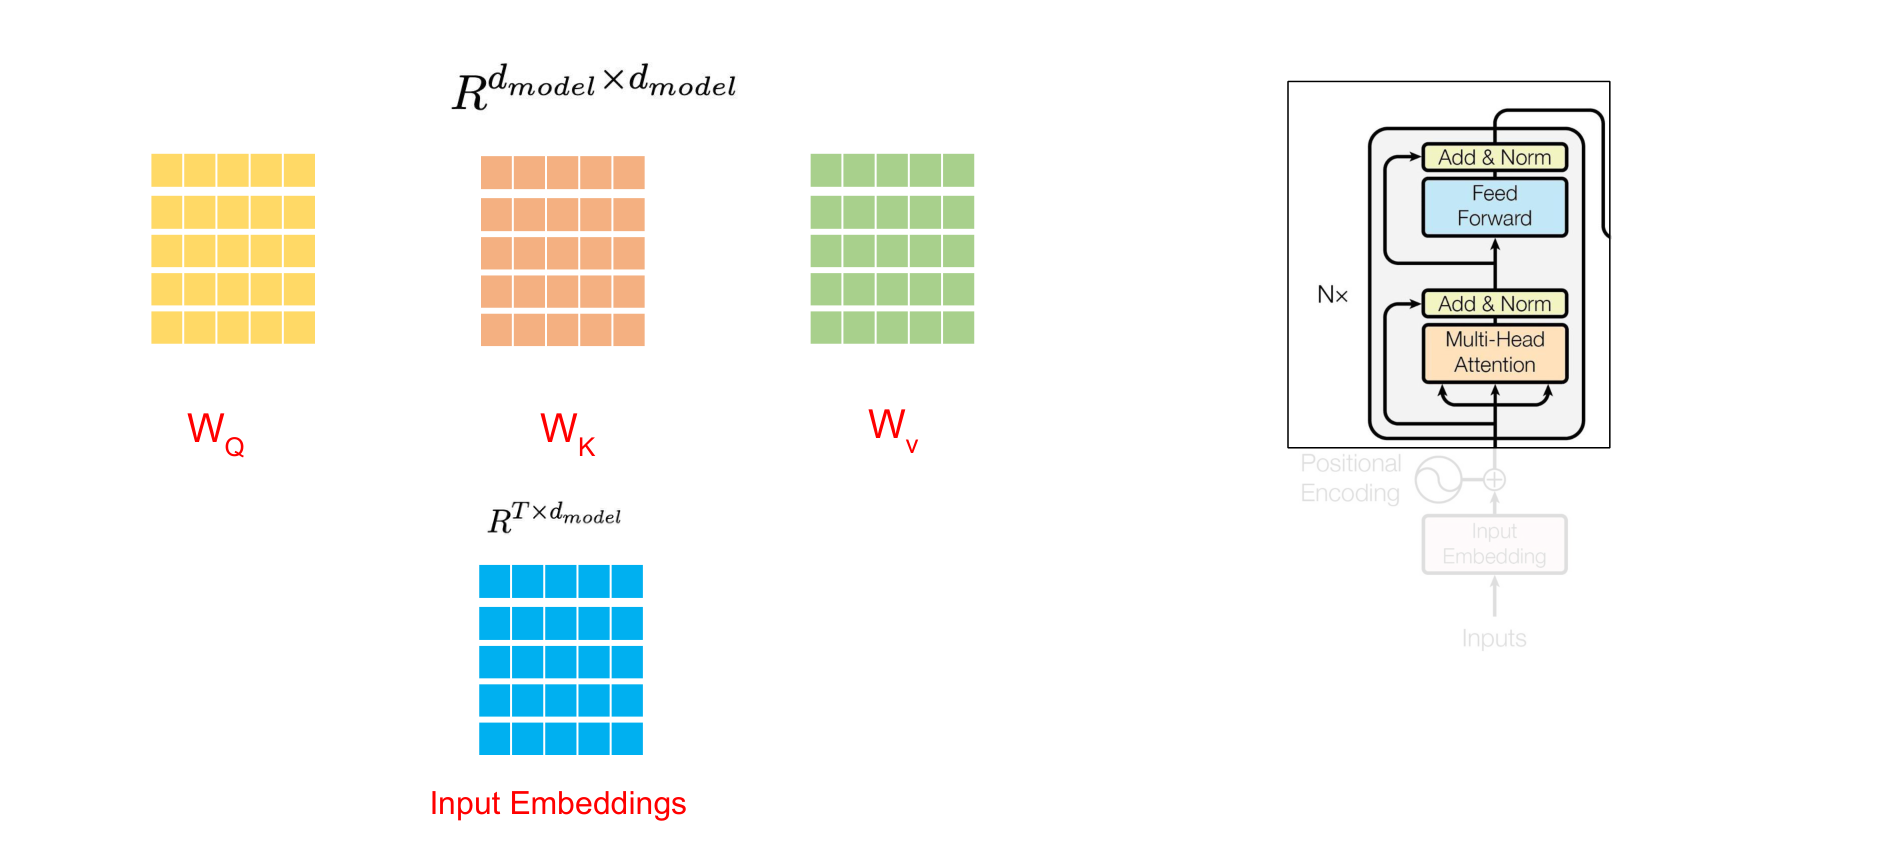
\includegraphics[width=\linewidth,height=0.75\paperheight,keepaspectratio]{images/introduction-to-transformers/transformer_weight_matrices_wq_wk_wv_embeddings_encoder.png}

  {\scriptsize Source: CMU 11-785, Lecture 19 ``Transformers,'' Spring 2024, slide 75.}
\end{frame}

